\documentclass[14pt]{beamer}
\usepackage[utf8]{inputenc}
\usepackage[T1]{fontenc}
\usepackage{lmodern}
\usepackage{ngerman}
\usepackage{amsmath}
\usepackage{amsfonts}
\usepackage{amssymb}
\usepackage{graphicx}
\usepackage{pgfplots}
\usepackage{geometry}
\usepackage{fancyhdr}
\usepackage{lastpage}
\usepackage{float}
\usepackage{tikz}
\usepackage[european,smartlabels,siunitx]{circuitikz}
\usetikzlibrary{calc,positioning}

%\graphicspath{{example_pictures/}}

\pgfdeclareimage[width = 1.5cm]{meinlogo}{Logo.png}
\usetheme{CambridgeUS}
\usecolortheme{seagull}
\begin{document}
	\author[Gruppe D]{Marcel Sandermann, Micha Beyer, Patrick Schlüter, Daniel Wolf}
	\title{Kantenerkennung}
	\subtitle{Projekt 1}
	\logo{\pgfuseimage{meinlogo}}
	\institute[HS OWL]{Hochschule Ostwestfalen Lippe}
	\date{31.10.2018}
	%\subject{was das}
	%\setbeamercovered{transparent}
	\setbeamertemplate{navigation symbols}{}
	
	
\begin{frame}
	\titlepage
\end{frame}
\begin{frame}
	\frametitle{Inhalt}
	\tableofcontents	
\end{frame}
\section{Einleitung}
\subsection{Problemstellung}
\begin{frame}
	\frametitle{Problemstellung}
	\begin{itemize}
		\item Scheinbar einfarbiges Bild
		\item Schlechter Kontrast	
	\end{itemize}
	\begin{columns}[c]
		\column{.3\textwidth}
		\begin{figure}
		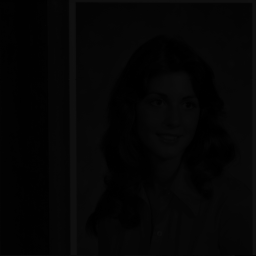
\includegraphics[width=0.8\linewidth]{GruppeDBild.png}
		\end{figure}
		\column{.3\textwidth}
		\begin{figure}
			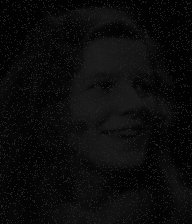
\includegraphics[width=0.8\linewidth]{enhance-me.png}
		\end{figure}
		\column{.3\textwidth}
		\begin{figure}
			
\includegraphics[width=0.8\linewidth]{GruppeBBild.png}
		\end{figure}		 	
	\end{columns}
		
\end{frame}

\section{Lösungsweg}
\subsection{Kontrastanpassung}

\begin{frame}
	\frametitle{Kontrastanpassung}	
	\begin{columns}
		\column{.6\linewidth}
		\begin{enumerate}
			\item $a_{low}\ \&\ a_{high}$ bestimmen
			\item Skalieren auf neuen Bereich 
		\end{enumerate}	
		\column{.4\linewidth}
		\begin{figure}
			\centering
			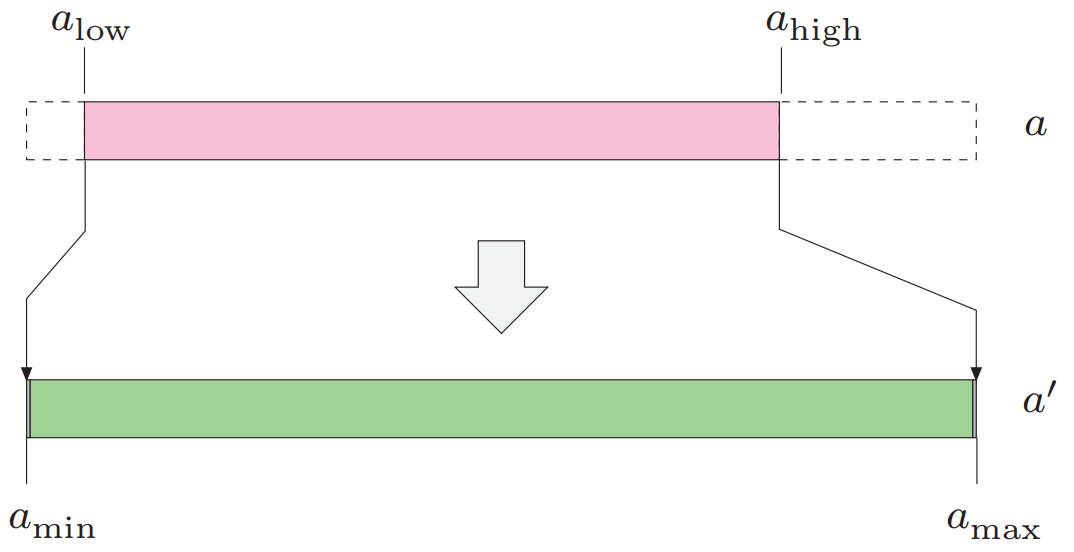
\includegraphics[width=\linewidth]{Kontrastanpassung.PNG}
		\end{figure}
	\end{columns}

	\begin{block}{Kontrastanpassung}
		\begin{equation*}
		f_{ac}=a_{min} (a - a_{low}) \frac{a_{max}-a_{min}}{a_{high}-a_{low}}
		\end{equation*}
	\end{block}		
		
	\end{frame}

\begin{frame}
	\frametitle{Kontrastanpassung}
	\begin{columns}[c]
		\column{.3\textwidth}
		\begin{figure}
			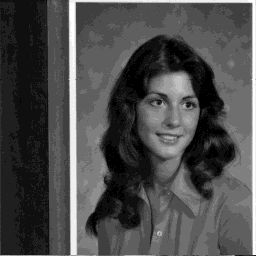
\includegraphics[width=0.8\linewidth]{GruppeDBild_2.png}
		\end{figure}
		\column{.3\textwidth}
		\begin{figure}
			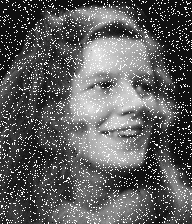
\includegraphics[width=0.8\linewidth]{enhance-me_2.png}
		\end{figure}
		\column{.3\textwidth}
		\begin{figure}
			
\includegraphics[width=0.8\linewidth]{GruppeBBild_2.png}
		\end{figure}		 	
	\end{columns}	
	\begin{itemize}
		\item Nur teilweise Erfolgreich
	\end{itemize}
\end{frame}

\begin{frame}
	\frametitle{Kontrastanpassung}
	\begin{figure}
		\centering
		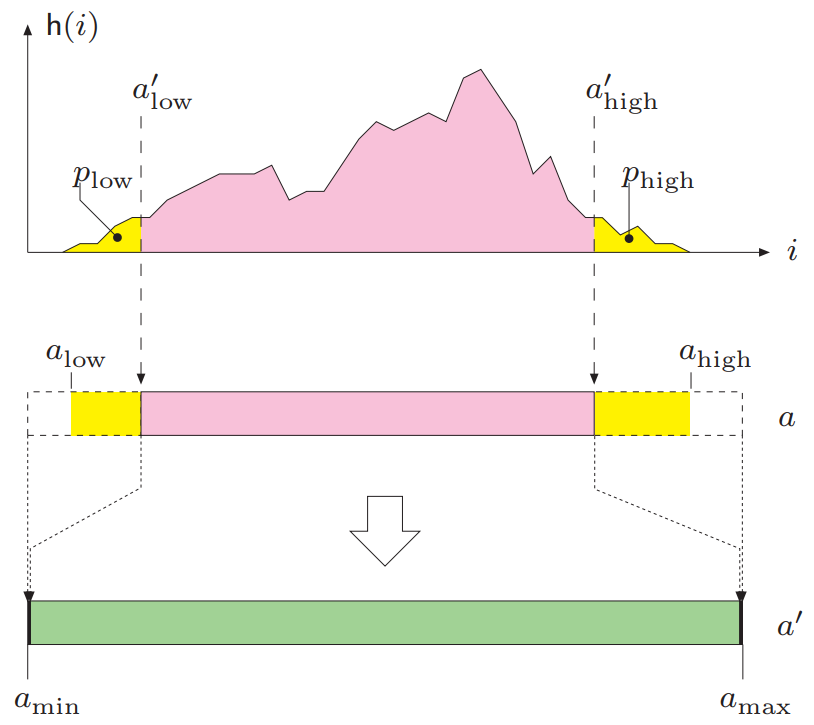
\includegraphics[width=0.7\linewidth]{Clipping.PNG}
	\end{figure}
\end{frame}

\begin{frame}
	\begin{block}{Erweiterte automatische Kontrastanpassung}	
		\begin{equation*}
		\small{
			f_{kont}=
			\begin{cases}
			a_{min}   			& \text{für } a \leq a'_{low}, \\
			a_{min} + (a-a'_{low})*\frac{a_{max}-a_{min}}{a'_{high}-a'_{low}}	& \text{für } a'_{low} < a < a'_{high}, \\
			a_{max}        		& \text{für } a \geq a'_{high}
			\end{cases}
		}
		\end{equation*}
	\end{block}
	\begin{itemize}
		\item Festlegung der Grenzwertewerte $a'_{low}\ \&\ a'_{high}$
	\end{itemize}

\end{frame}

\begin{frame}
	\frametitle{Kontrastanpassung}
	\begin{columns}[c]
		\column{.3\textwidth}
		\begin{figure}
			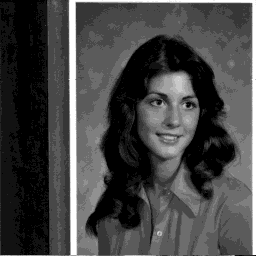
\includegraphics[width=0.8\linewidth]{GruppeDBild_3.png}
		\end{figure}
		\column{.3\textwidth}
		\begin{figure}
			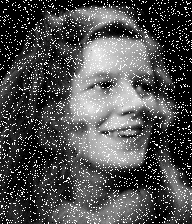
\includegraphics[width=0.8\linewidth]{enhance-me_3.png}
		\end{figure}
		\column{.3\textwidth}
		\begin{figure}
			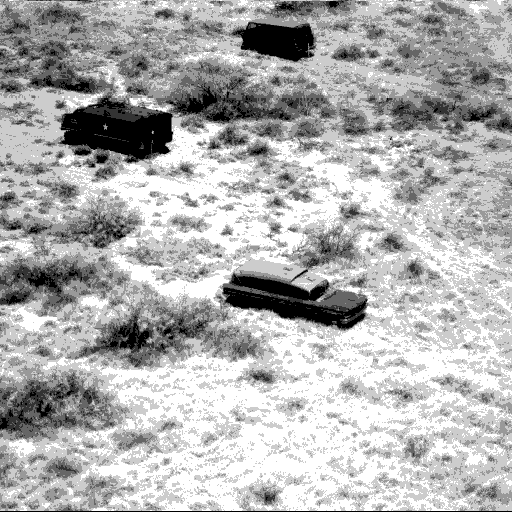
\includegraphics[width=0.8\linewidth]{GruppeBBild_3.png}
		\end{figure}		 	
	\end{columns}	
	\begin{itemize}
		\item Besser
	\end{itemize}
\end{frame}

\section{Fazit}

\begin{frame}
	\frametitle{Fazit}
	\begin{itemize}
		\item Einfache Kontrastanpassung führt selten zu brauchbarem Ergebnis
		\item Clipping verbessert Ergebnis
		\item Grenzwerte müssen besser bestimmt werden		
	\end{itemize}
\end{frame}

\section*{}

\begin{frame}
	\Large\centering{Vielen Dank für eure Aufmerksamkeit}	
	\newline
	\begin{block}{Quellen}
		\small{	
		\begin{thebibliography}{99} % Beamer does not support BibTeX so references must be inserted manually as below
			\bibitem[Burger, Burge, 2015]{p1} Wilhelm Burger, Mark James Burge (2015)
			\newblock Digitale Bildverarbeitung: Eine algorithmische Einführung mit Java
			%\newblock \emph{Journal Name} 12(3), 45 -- 678.
		\end{thebibliography}
		}
	\end{block}
\end{frame}

\end{document}